%\documentclass[preprint,tightenlines,showpacs,showkeys,floatfix,
%nofootinbib,superscriptaddress,fleqn]{revtex4} 
\documentclass[floatfix,nofootinbib,superscriptaddress,fleqn,preprint]{revtex4-2}  
%\documentclass[aps,epsfig,tightlines,fleqn]{revtex4}
\usepackage[utf]{kotex}
\usepackage[HWP]{dhucs-interword}
\usepackage[dvips]{color}
\usepackage{graphicx}
\usepackage{bm}
%\usepackage{fancyhdr}
%\usepackage{dcolumn}
\usepackage{defcolor}
\usepackage{amsmath}
\usepackage{amsfonts}
\usepackage{amssymb}
\usepackage{amscd}
\usepackage{amsthm}
\usepackage[utf8]{inputenc}
 \usepackage{setspace}
%\pagestyle{fancy}

\begin{document}

\title{\Large 2022년 1학기 물리학 I: Quiz 4}
\author{김현철\footnote{Office: 5S-436D (면담시간 매주
    화요일-16:00$\sim$20:00)}} 
\email{hchkim@inha.ac.kr}
\affiliation{Hadron Theory Group, Department of Physics, Inha University,
Incheon 402-751, Republic of Korea }
\date{Spring semester, 2022}
\maketitle

\noindent {\bf 문제 1 [10pt]} 
그림~\ref{fig:1}과 같이 어떤 사람이 건물
꼭대기에서 수평에서부터 $30^\circ$의 각도로, 20.0 m/s의 속도로
공을 던졌다. 건물 
바닥에서 공을 던진 곳까지 높이는 45.0 m이다. 
\begin{figure}[ht]
  \centering
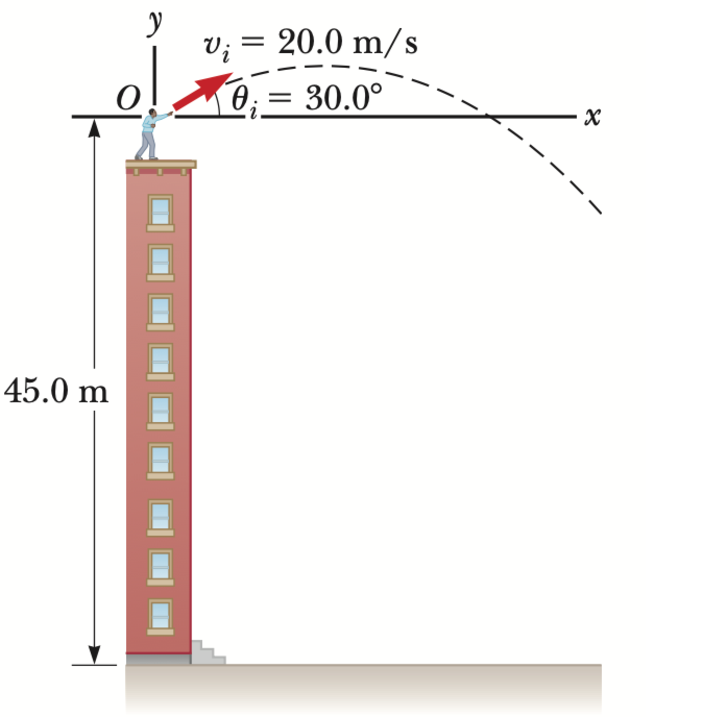
\includegraphics[scale=0.6]{Qfig4-2.pdf}  
  \caption{문제 2}
  \label{fig:1}
\end{figure}
\begin{itemize}
\item[(가)] 공이 지면에 닿을 때까지 걸린 시간을 구하여라.
\item[(나)] 공이 지면에 닿을 때 속력을 구하여라. (이 문제에서는 계산기를
  쓰셔도 무방합니다.)
\end{itemize}
\vspace{0.2cm}

\noindent \textbf{풀이:}
초기 위치는 $x_i=y_i=0$, $y$ 성분의 나중
위치는 $y_f=-45.0$ m이고, $a_y=-g$, $v_i=20.0$ m/s이다. 따라서 속도는
각각
\begin{align}
v_{xi}  &=v_i\cos\theta_i =(20.0\,\mathrm{m/s})(\cos30.0^\circ) = 17.3
          \,\mathrm{m/s},\cr
v_{yi} &= v_i\sin\theta_i = (20.0\,\mathrm{m/s})(\sin30.0^\circ) =
         10.0    \,\mathrm{m/s}           
\end{align}
가 된다. 이제 $y_f$는
\begin{align}
  \label{eq:5}
 y_f = y_i + v_{yi} t - \frac12 g t^2 
\end{align}
가 된다. 이 식은 아래와 같이 $t$에 대한 이차 방정식으로 쓸 수 있다.
\begin{align}
  \label{eq:6}
  \frac12 g t^2 -v_{yi}t +(y_f-y_i) =
  \left(\frac{9.80\,\mathrm{m/s^2}}{2}\right) t^2 -
  (10.0\,\mathrm{m/s})   t -45.0\,\mathrm{m} 
\end{align}
이므로, 근의 해 공식을 쓰자.
\begin{align}
t = \frac{-b\pm\sqrt{b^2 - 4ac}}{2a}  
\end{align}
여기서
\begin{align}
  \label{eq:8}
  a = 4.90\,\mathrm{m/s^2},\;\;\; b = -10.0\,\mathrm{m/s} ,\;\;\;
  c= -45.0\,\mathrm{m}
\end{align}
이므로,
\begin{align}
  \label{eq:9}
  t_1 &= \frac{-(10.0\,\mathrm{m/s})+\sqrt{(-10.0\,\mathrm{m/s})^2
  -  4(4.90\,\mathrm{m/s^2})(-45.0\,\mathrm{m})}}
        {2(4.90\,\mathrm{m/s^2})}  = 4.22\,\mathrm{s}, \cr
 t_2 &= \frac{-(10.0\,\mathrm{m/s})-\sqrt{(-10.0\,\mathrm{m/s})^2
  -  4(4.90\,\mathrm{m/s^2})(-45.0\,\mathrm{m})}}
        {2(4.90\,\mathrm{m/s^2})}  = -2.18\,\mathrm{s},        
\end{align}
여기서 $t_2<0$은 우리가 원하는 시간이 아니다. 따라서 답은 
\begin{align}
t = 4.22\,\mathrm{s}  
\end{align}
이다.

\noindent (나) 공이 땅에 닿을 때 속도의 각각의 성분은 
\begin{align}
  \label{eq:11}
  v_{xf} = v_{xi} ,\;\;\;
  v_{yf} = v_{yi} -gt 
\end{align}
이다. 여기에 앞에서 구한 수치를 대입하면,
\begin{align}
  v_{xf} =17.3\,\mathrm{m/s},\;\;\;
  v_{yf} = 10.0\,\mathrm{m/s} -
  (9.8\,\mathrm{m/s^2})(4.218\,\mathrm{s}) = -31.3\,\mathrm{m/s} 
\end{align}
가 되고, 속력은
\begin{align}
  \label{eq:13}
v = \sqrt{v_{xf}^2 +v_{yf}^2} = \sqrt{(17.3\,\mathrm{m/s})^2
  +(-31.3\,\mathrm{m/s})^2} =35.8\,\mathrm{m/s}  
\end{align}
가 된다.

\noindent 
{\color{red} 주의! 수치 계산을 할 때, 유효숫자는 가장 마지막에
  따져주는 게 좋다.}


\vspace{1cm}
\noindent {\bf 문제 2 [20pt]} 초기 위치 $x_0$, 초기 속력 $v_0$이
주어졌을 때, 아래의 식
\begin{align}
  \label{eq:1}
v^2 - v_0^2 = 2a(x-x_0)  
\end{align}
을 다음과 같이 유도해보자. 순간 가속도는
\begin{align}
  \label{eq:2}
a = \frac{dv}{dt}
\end{align}
와 같이 주어진다. \eqref{eq:2}의 양변에 속력 $v$를 곱한 식에서부터
\eqref{eq:1}을 유도하여라. (적분을 이용하여야 한다는 점을 명심하여라.)
\vspace{0.2cm}

\noindent \textbf{풀이:}
$a$와 $v$를 곱한 양을 우선 적으면,
\begin{align}
  \label{eq:3}
  av &= a \frac{dx}{dt} = v \frac{dv}{dt} 
\end{align}
이 된다. 양변에 $dt$를 곱해주면, 
\begin{align}
  \label{eq:4}
a dx = v dv  
\end{align}
가 되고, $a$는 일정한 가속도이므로 양변을 적분하면, 
\begin{align}
a \int_{x_{0}}^{x}  dx^{\prime} &= a(x-x_{0}) 
  = \int_{v_{0}}^{v} v^{\prime} dv^{\prime} = \frac{1}{2} (v^{2} -
              v_{0}^{2}) 
\end{align}
을 얻고,
\begin{align}
  \label{eq:7}
v^2-v_0^2 = a(x-x_0)   
\end{align}
를 얻는다. 
\vspace{1cm}

\noindent {\bf 문제 3 [10pt]} 
스키 점프 선수가 트랙의 수평면에 도달해서 수평방향으로 도약을 했다. 이
때 속력은 20.0 m/s였다. 그리고 수평면과 경사면 사이의 각은
$35.0^\circ$였다. 이 선수는 어느 지점에 착지했을까?  
\begin{figure}[ht]
  \centering
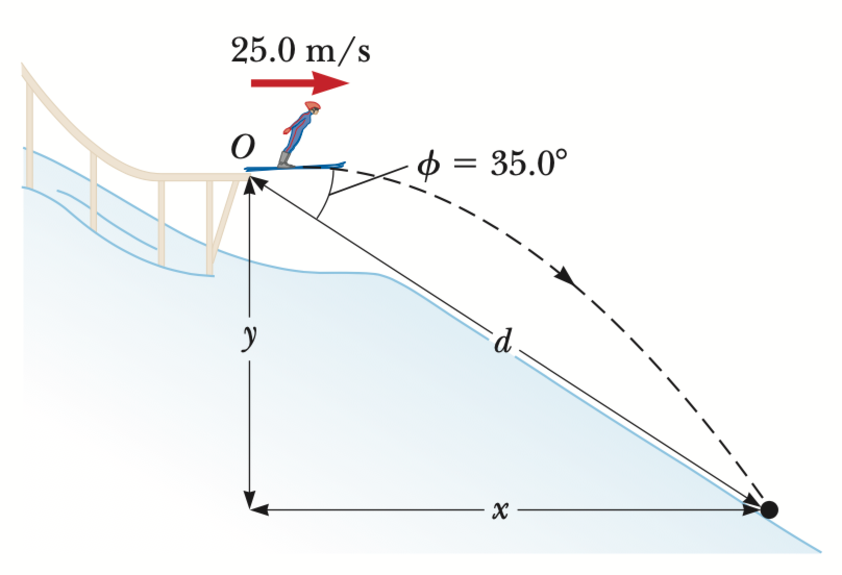
\includegraphics[scale=0.6]{Qfig4-3.pdf}  
  \caption{문제 3}
  \label{fig:2}
\end{figure}
\vspace{0.2cm}

\noindent \textbf{풀이:}
초기 속도는 $v_{xi}=25.0\,\mathrm{m/s}$,
$v_{yi}=0$이고, 스키 선수가 착지하는 지점의 위치는 
\begin{align}
  \label{eq:14}
  x_f = d\cos\phi,\;\;\; y_f = -d\sin\phi
\end{align}
이다. 여기서 $y_f$가 음의 값이 되는 이유는 스키선수가 점프하는 순간의
지점을 원점으로 잡았기 때문이다.
따라서 
\begin{align}
  \label{eq:15}
x_f = v_{xi} t,\;\;\; y_f = v_{yi} t - \frac12 gt^2  
\end{align}
이 되므로,
\begin{align}
  \label{eq:16}
  d\cos\phi = v_{xi} t,\;\;\;
  -d\sin\phi = -\frac12 g t^2
\end{align}
이 된다. 여기서 $d$를 구하기 위해 $t$를 소거하면,
\begin{align}
  \label{eq:17}
d = \frac{2v_{xi}^2 \sin\phi}{g\cos^2\phi} =
  \frac{2(25.0\,\mathrm{m/s})^2 \sin
  35.0^\circ}{(9.80\,\mathrm{m/s^2})\cos^235.0^\circ } =
  109\,\mathrm{m}   
\end{align}
가 된다. 따라서
\begin{align}
  \label{eq:18}
x_f &= d\cos\phi = (109\,\mathrm{m})\cos35.0^\circ = 89.3\,\mathrm{m},
      \cr
y_f &= -d\sin\phi = -(109\,\mathrm{m})\sin35.0^\circ =
      -62.5\,\mathrm{m}
\end{align}
가 바로 스키 선수가 착지하는 위치다. 


\vspace{1cm}

\noindent {\bf 문제 4 [10pt]} 높이가 $y_0=15.0$ m인 건물이 있다. 이 건물
꼭대기에서 $v_0=10.0$ m/s의 속력으로 위로 공을 쏘아올렸다. 
\begin{figure}[ht]
  \centering
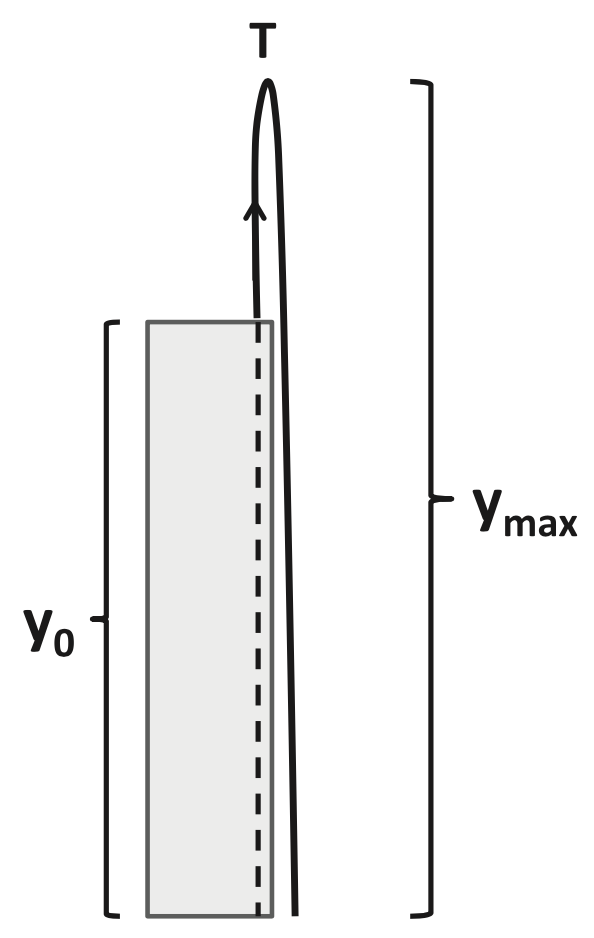
\includegraphics[scale=0.5]{Qfig4-4-20210312.png}  
  \caption{문제 4}
  \label{fig:4}
\end{figure}
그림~\ref{fig:4}에 보여주는 $y_{\mathrm{max}}$를 구하여라. 
\vspace{0.2cm}

\noindent \textbf{풀이:}
물체는 아래 방향으로 일정한 중력가속도 $g$를 받고 있으므로, 
위로 쏘아 올려진 물체의 속도와 높이는 다음과 같이 나타 낼 수 있다.
\begin{align}
 \label{4-1}
v_{y}(t) &= v_{0} - gt \\
 \label{4-2}
y(t) &= y_{0} + v_{0}t - \frac{1}{2} g t^{2}.
\end{align}
물체가 최고높이에 도달한 순간 물체의 속력은 $0 \; \mathrm{m/s}$가 
되므로 최고높이에 도달할때의 시간을 $T$라 하면, 최고높이는 다음과 같이 나타 낼 수 있다.
\begin{align}
 \label{4-3}
v_{y}(T) &= 0 = v_{0} - gT \rightarrow T = \frac{v_{0}}{g} \\
 \label{4-4}
y(T) &= y_\mathrm{max} = y_{0} + v_{0}T - \frac{1}{2} g T^{2} 
  = y_{0} + \frac{v_{0}^{2}}{g} - \frac{v_{0}^{2}}{2g}
  = y_{0} + \frac{v_{0}^{2}}{2g}.
\end{align}
주어진 값을 대입하여 $y_\mathrm{max}$를 구하면 다음과 같다.
\begin{align}
 \label{4-5}
y_\mathrm{max} &= 15.0 \; \mathrm{m} + \frac{(10.0 \; \mathrm{m/s})^{2}}{2(9.8 \; \mathrm{m/s^{2}})}
  = 20.1 \; \mathrm{m}
\end{align}


\end{document}